\chapter{Additional Results}\label{app:additional-results}

In this appendix, we justify the bounded hyperparameter grids over which the
regularization penalties are selected in the empirical analysis of
\Cref{chap:backtest-analysis}. In
\Cref{app:hyperparameter-sensitivity} we describe the sensitivity analysis used to
determine these bounds, following a similar approach as
\cite{RegularizedMultiCurrencyExpectedShortfallPortfolios}.

TODO: Summarize the sparsity analysis and its purpose.


\section{Hyperparameter Grids} \label{app:hyperparameter-sensitivity}

The regularized overlay and joint programs have four penalties in the objective, the asset penalties $\lambda_1^a$ and $\lambda_2^a$ and
the currency penalties $\lambda_1^c$ and $\lambda_2^c$, while the asset-only optimizers, Full and Zero, only have the
two asset penalties. In the backtests, the penalties are selected at every rebalancing date by the grid search described in
\Cref{sec:backtesting-framework}. The grid we optimize over is the Cartesian product of the penalty values, with $256$ points for the overlay and
joint programs and $16$ points for Full and Zero programs. The asset leverage
limit is fixed at $\ell^a = 2$ for all the programs, and the confidence level of Expected Shortfall and second-order Expected Shortfall at
$\beta = 0.8$.
 
As the penalty sizes are increased, the optimal weights approach a limiting
allocation, and beyond some threshold a further increase leaves the solution unchanged. A grid whose
largest value lies past that threshold covers the whole range of regularization, and extending it further would only
increase the computational cost of the grid search.

To locate this threshold, we use a similar approach to \cite{RegularizedMultiCurrencyExpectedShortfallPortfolios} and analyze each penalty
$\lambda \in \{\lambda_1^a, \lambda_2^a, \lambda_1^c, \lambda_2^c\}$ on its own, holding the other three fixed at zero. We consider an
increasing sequence $0 = \lambda_0 < \lambda_1 < \dots < \lambda_K$.
Let $\bm{x}_t(\lambda_n)$ and $\bm{\psi}_t(\lambda_n)$ denote the optimal asset weights and currency exposures at
$\lambda_n$. The marginal effect of the step from $\lambda_{n-1}$ to $\lambda_n$ is measured in the supremum norm
\begin{equation*} 
\begin{aligned}
    d_n^a &= \left\| \bm{x}_t(\lambda_n) - \bm{x}_t(\lambda_{n-1}) \right\|_\infty
    \quad \text{for } \lambda \in \{\lambda_1^a, \lambda_2^a\}, \\
    d_n^c &= \left\| \bm{\psi}_t(\lambda_n) - \bm{\psi}_t(\lambda_{n-1}) \right\|_\infty
    \quad \text{for } \lambda \in \{\lambda_1^c, \lambda_2^c\}.
\end{aligned}
\end{equation*} 

The two penalty types approach their limits in different ways. Under an $L^1$ penalty, the weights reach their limit
at a finite value of the penalty, a long-only portfolio for the asset weights and a zero overlay for the currency
exposures, and do not change as the penalty is increased further. An $L^2$ penalty
instead shrinks the weights smoothly toward their limit, the equally weighted portfolio for the asset weights and a
zero overlay for the currency exposures, and reaches it only asymptotically, so its marginal effect decays gradually
without vanishing \cite{HastieTibshiraniFriedman2009}. For this reason, we report alongside $d_n^a$ and $d_n^c$ the
portfolio exposure, $\|\bm{x}_t(\lambda_n)\|_1$ for the asset penalties and $\|\bm{\psi}_t(\lambda_n)\|_1$ for the
currency penalties.

The analysis is carried out for the regularized overlay and joint programs of each risk measure on the first lookback
window of the small universe, which spans July 1990 to June 2000 and contains $2{,}610$ daily observations. To account for sampling error, each reported quantity is averaged over five bootstrap replications of this
window, each constructed by resampling its daily observations with replacement.

We visualize the results for the regularized variance programs, whose marginal effects and exposures are shown in
\Cref{fig:hyperparameter-sensitivity-mv-marginal,fig:hyperparameter-sensitivity-mv}. The overlay and joint programs
behave very similarly. The difference between the two penalty types is clearest in \Cref{fig:hyperparameter-sensitivity-mv-marginal}. Once the
weights reach their limit under an $L^1$ penalty, the marginal effect has a sudden drop, to zero for the currency
exposures and by more than two orders of magnitude for the asset weights. 
The $L^2$ penalties do not exhibit such a drop, which is why their largest grid values are interpreted from the
exposure in \Cref{fig:hyperparameter-sensitivity-mv} instead.

For both asset penalties, exposure falls from slightly below the leverage limit to one. 
Once the portfolio becomes long-only, the $L^1$ penalty equals the constant $\lambda_1^a$, so the solution stops changing.
We set the largest grid value to $5 \times 10^{-5}$, by which this has happened.
As discussed in \Cref{app:mv_regularization}, the $L^2$ penalty instead shrinks the covariance estimate toward a scaled identity matrix, since
$\bm{x}_t^\top \bm{\Sigma}_t \bm{x}_t + \lambda_2^a \|\bm{x}_t\|_2^2 = \bm{x}_t^\top (\bm{\Sigma}_t + \lambda_2^a \bm{I}_N)
\bm{x}_t$, so the weights move toward the equally weighted portfolio. We set the largest grid value to $10^{-2}$, by which there are no longer 
any short positions.

The currency exposures carry neither a budget nor a leverage constraint, so $\bm{\psi}_t$ shrinks to zero. Under
$\lambda_1^c$, the currency exposures disappear at $5 \times 10^{-5}$. Under $\lambda_2^c$, they never fully disappear,
so we determine the largest grid value as the point at which the overlay becomes negligible. From $1.7 \times 10^{-3}$
onward, less than one percent of the unpenalized currency exposure remains, and we set the largest grid value to
$2 \times 10^{-3}$.

\begin{figure}[p]
    \centering
    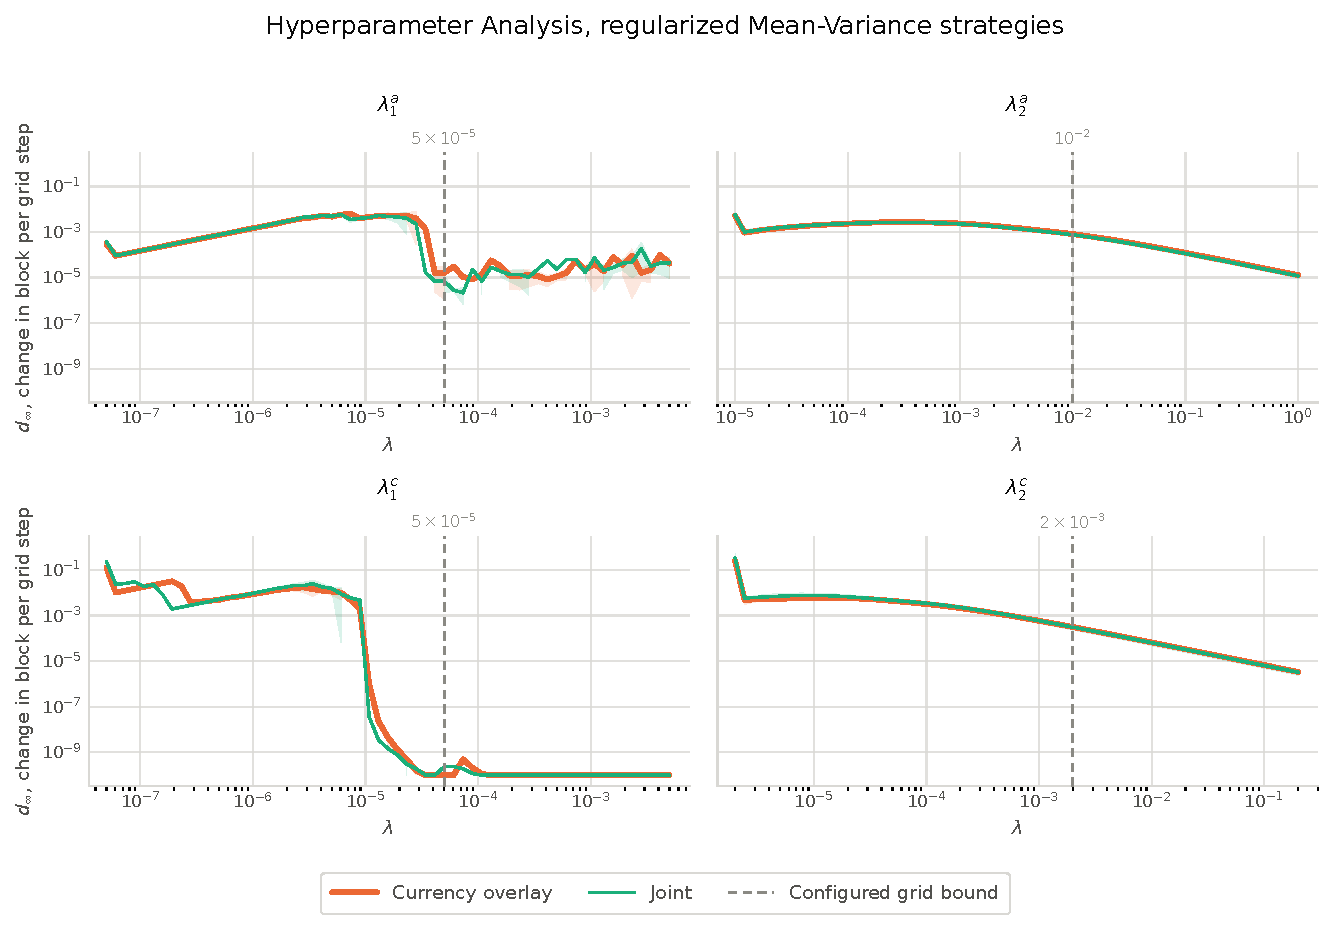
\includegraphics[width=0.9\textwidth]{../results/figures/boundary_plots/mv_top10_dinf.pdf}
    \caption{Marginal effect of each penalty for the regularized variance overlay and joint programs. The upper panels
    report $d_n^a$ for the asset penalties and the lower panels $d_n^c$ for the currency penalties. The dashed lines mark
    the largest value of each grid in \Cref{tab:hypergrid}. Averaged over five bootstrap replications of the first
    lookback window of the small universe (top-10).}
    \label{fig:hyperparameter-sensitivity-mv-marginal}

    \vspace{1.5em}

    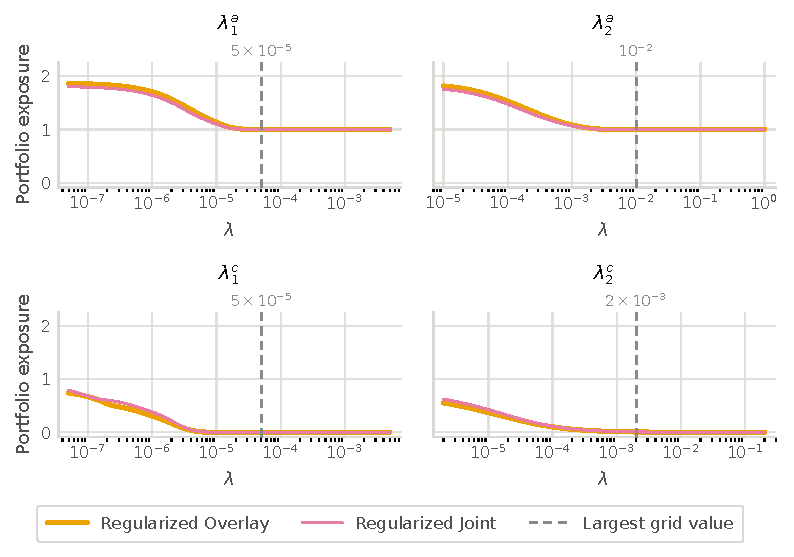
\includegraphics[width=0.9\textwidth]{../results/figures/boundary_plots/mv_top10_gross.pdf}
    \caption{Portfolio exposure as a function of each penalty for the regularized variance overlay and joint programs.
    The upper panels report $\|\bm{x}_t\|_1$ for the asset penalties and the lower panels $\|\bm{\psi}_t\|_1$ for the
    currency penalties. The dashed lines mark the largest value of each grid in \Cref{tab:hypergrid}. Averaged over five
    bootstrap replications of the first lookback window of the small universe (top-10).}
    \label{fig:hyperparameter-sensitivity-mv}
\end{figure}

We perform the same analysis for the regularized overlay and joint programs of the other four risk measures. 
They show the same pattern as the variance
programs. Both asset penalties reduce the asset exposure to one, the currency $L^1$ penalty removes the currency
exposures at a finite value, and the currency $L^2$ penalty shrinks them smoothly toward zero. 

On the basis of this analysis, we construct the grids reported in \Cref{tab:hypergrid}. 
The upper bounds of the asset $L^1$ penalty for variance and
semi-variance are set to $5 \times 10^{-5}$
and $10^{-4}$, while those for MAD, Expected Shortfall and second-order Expected Shortfall are set to $2.5 \times 10^{-3}$, $5 \times 10^{-3}$ and $10^{-1}$.
The asset penalty grids
of the variance and semi-variance programs lie one to three orders of magnitude below those of the other risk measures. This 
is because they are measured in squared returns.

\begin{table}[htbp]
\centering
\small
\begin{tabular}{llll}
\toprule
Risk measure & Penalty & Description & Range \\
\midrule
Variance      & $\lambda_1^a$ & Asset $L^1$ penalty    & $[0,\ 5\times10^{-5}]$ \\
              & $\lambda_2^a$ & Asset $L^2$ penalty    & $[0,\ 10^{-2}]$ \\
              & $\lambda_1^c$ & Currency $L^1$ penalty & $[0,\ 5\times10^{-5}]$ \\
              & $\lambda_2^c$ & Currency $L^2$ penalty & $[0,\ 2\times10^{-3}]$ \\
\midrule
Semi-Variance & $\lambda_1^a$ & Asset $L^1$ penalty    & $[0,\ 10^{-4}]$ \\
              & $\lambda_2^a$ & Asset $L^2$ penalty    & $[0,\ 5\times10^{-2}]$ \\
              & $\lambda_1^c$ & Currency $L^1$ penalty & $[0,\ 2.5\times10^{-5}]$ \\
              & $\lambda_2^c$ & Currency $L^2$ penalty & $[0,\ 10^{-3}]$ \\
\midrule
MAD           & $\lambda_1^a$ & Asset $L^1$ penalty    & $[0,\ 2.5\times10^{-3}]$ \\
              & $\lambda_2^a$ & Asset $L^2$ penalty    & $[0,\ 1]$ \\
              & $\lambda_1^c$ & Currency $L^1$ penalty & $[0,\ 1.5\times10^{-3}]$ \\
              & $\lambda_2^c$ & Currency $L^2$ penalty & $[0,\ 2.5\times10^{-1}]$ \\
\midrule
ES            & $\lambda_1^a$ & Asset $L^1$ penalty    & $[0,\ 5\times10^{-3}]$ \\
              & $\lambda_2^a$ & Asset $L^2$ penalty    & $[0,\ 3]$ \\
              & $\lambda_1^c$ & Currency $L^1$ penalty & $[0,\ 5\times10^{-4}]$ \\
              & $\lambda_2^c$ & Currency $L^2$ penalty & $[0,\ 5\times10^{-5}]$ \\
\midrule
SOES          & $\lambda_1^a$ & Asset $L^1$ penalty    & $[0,\ 10^{-1}]$ \\
              & $\lambda_2^a$ & Asset $L^2$ penalty    & $[0,\ 15]$ \\
              & $\lambda_1^c$ & Currency $L^1$ penalty & $[0,\ 10^{-2}]$ \\
              & $\lambda_2^c$ & Currency $L^2$ penalty & $[0,\ 1]$ \\
\bottomrule
\end{tabular}
\caption{Ranges of the hyperparameter grids of the regularized programs.}
\label{tab:hypergrid}
\end{table}

\newpage
\section{Portfolio Sparsity Analysis} \label{app:portfolio-sparsity}

\subsection*{Sparsity of the Regularized Expected Shortfall Optimizers} \label{app:sparsity-es}

\begin{figure}[httb]
    \centering
    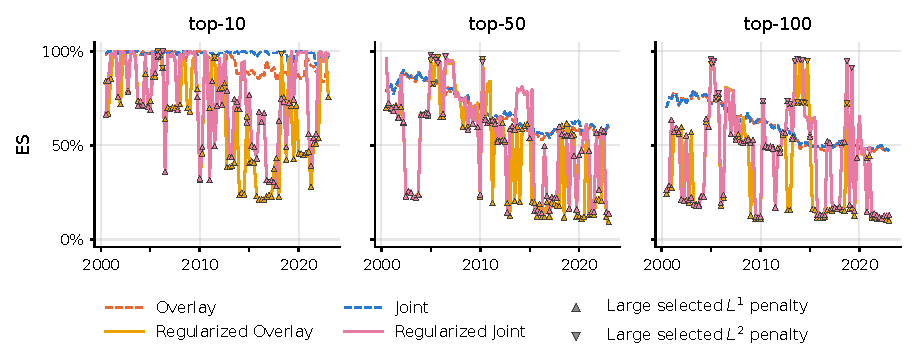
\includegraphics[width=1\textwidth]{../results/figures/sparsity_analysis/normal/es_assets.pdf}
    \caption{Sparsity of the regularized Expected Shortfall currency overlay and joint optimizers.}
    \label{fig:sparsity-es}
\end{figure}

Figure \ref{fig:sparsity-es} reports the share of the investable universe held at each rebalance date.

Regularization stabilizes the weight vector conditional on the penalty coefficients, 
but those coefficients are themselves re-selected at every rebalance date. 
The number of active positions is sensitive to this recalibration, an L1-dominant selection
 sets weights to zero and yields a concentrated portfolio, whereas an L2-dominant selection 
 shrinks all weights toward the equally weighted portfolio. 
 The oscillation therefore reflects the validation criterion alternating between these two regimes 
 across quarters, not instability in the optimizer itself. The unregularized problem has no such 
 degree of freedom. Its support is determined primarily by the leverage limit.

\subsection*{Sparsity of the Regularized Mean-Variance Optimizers} \label{app:sparsity-mv}

\begin{figure}[httb]
    \centering
    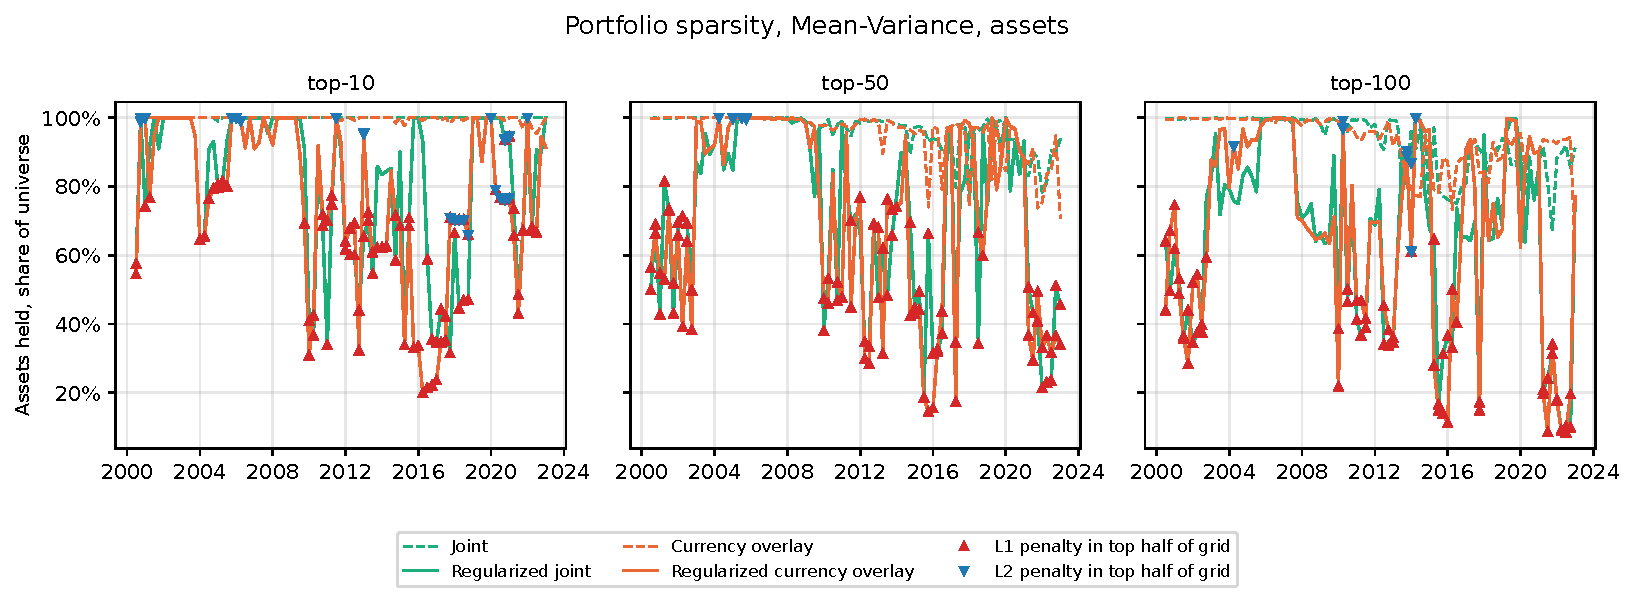
\includegraphics[width=1\textwidth]{../results/figures/sparsity_analysis/normal/mv_assets.pdf}
    \caption{Sparsity of the regularized Mean-Variance currency overlay and joint optimizers.}
    \label{fig:sparsity-mv}
\end{figure}
\subsection*{Sparsity of the Regularized Mean Absolute Deviation Optimizers} \label{app:sparsity-mad}


\section{Risk Aversion Instability under Mean Variance Optimization} \label{app:instability-mv}

In \Cref{chap:backtest-analysis} we report backtest results for the mean-variance optimizers under infinite risk aversion, 
which corresponds to the minimum variance problem. We do this because the mean-variance optimization problem is 
is unstable under finite risk aversion \cite{DeMiguel et al. 2009}. We showcase this by runnign the 
regularized overlay and joint optimizers under finite risk aversion on the top 10 universe and report the results in 
\ref{tab:instability-mv}. 

\begin{table}[ht]
    \centering 
    \scalebox{0.82}{%
    \begin{tabular}{lcc}
        \toprule
        \multicolumn{3}{c}{\textbf{Mean-Variance Optimizers under Finite Risk Aversion}} \\
        \midrule
        \textbf{Metric} &       \textbf{Overlay} &      \textbf{Joint} \\
        \midrule
        ES (\%)                   & 2.07                  & 2.20    \\
        Vol (\%)                  & 26.50                 & 28.54    \\
        MD (\%)                   & 70.15                 & 69.31   \\
        SR                        & 0.10                  & 0.11    \\
        SOR                       & 0.07                  & 0.15    \\
        ESR                       & 0.08                  & 0.09    \\   
        $\text{Turnover}^a$       & 1.82                  & 1.84    \\
        $\text{Turnover}^c$       & 19.04                 & 18.60    \\
        \bottomrule
    \end{tabular}
    }
    \caption{Performance metrics for the regularized mean-variance currency overlay and joint optimizers under finite risk aversion on the top 10 universe.}
    \label{tab:instability-mv}
\end{table}

We can see from table \ref{tab:instability-mv} that the performance of the optimizers is highly unstable and results in poor out of sample performance of the portfolios.
Two 

\section{Additional Backtest Performance Results} \label{app:additional-backtest-results}

\begin{table}%[htbp]
  \centering 
  \scalebox{0.82}{%
  \begin{tabular}{lcccccccc}
    \toprule
    \multicolumn{8}{c}{\textbf{Panel A: Small Investment Universe (top 10 stocks per economy)}} \\
    \midrule
    \textbf{Metric} & \textbf{Equal Weight} & \textbf{Assets-Full} & \textbf{Assets-Zero} & \textbf{Overlay} & \textbf{Overlay-Reg} & \textbf{Joint} & \textbf{Joint-Reg}\\
    \midrule
    ES (\%)                   & 1.15                 & 0.71                    & 0.98             & 0.69                & 0.67            & 0.67                & 0.66        \\
    Vol (\%)                  & 13.96                & 8.51                    & 11.84            & 8.18                & 7.99            & 7.97                & 7.85        \\
    MD (\%)                   & 54.76                & 30.81                   & 44.28            & 29.31               & 29.77           & 28.31               & 28.89       \\
    SR                        & 0.12                 & 0.10                    & 0.21             & 0.08                & 0.13            & 0.08                & 0.17        \\
    SOR                       & 0.17                 & 0.13                    & 0.28             & 0.10                & 0.18            & 0.11                & 0.23        \\
    ESR                       & 0.09                 & 0.08                    & 0.15             & 0.06                & 0.10            & 0.06                & 0.13        \\
    $\text{Turnover}^a$       & 0.29                 & 1.27                    & 1.23             & 1.30                & 1.06            & 1.27                & 1.15        \\
    $\text{Turnover}^c$       & 0.92                 & 0.93                    & 0                & 2.39                & 1.67            & 2.98                & 1.77        \\
    \midrule
    \multicolumn{8}{c}{\textbf{Panel B: Medium Investment Universe (top 50 stocks per economy)}} \\
    \midrule
    \textbf{Metric} & \textbf{Equal Weight} & \textbf{Assets-Full} & \textbf{Assets-Zero} & \textbf{Overlay} & \textbf{Overlay-Reg} & \textbf{Joint} & \textbf{Joint-Reg}\\
    \midrule
    ES (\%)                   & 1.04                    & 0.43                & 0.80              & 0.44              & 0.42             & 0.44                & 0.42    \\
    Vol (\%)                  & 12.50                   & 5.84                & 9.87              & 5.68              & 5.73             & 5.53                & 5.58    \\
    MD (\%)                   & 55.74                   & 38.54               & 42.37             & 38.59             & 38.56            & 38.84               & 36.38   \\
    SR                        & 0.32                    & 0.56                & 0.45              & 0.56              & 0.55             & 0.54                & 0.55    \\
    SOR                       & 0.44                    & 0.77                & 0.64              & 0.75              & 0.77             & 0.73                & 0.76    \\
    ESR                       & 0.24                    & 0.48                & 0.36              & 0.45              & 0.48             & 0.43                & 0.46    \\
    $\text{Turnover}^a$       & 0.27                    & 1.60                & 1.58              & 1.78              & 1.52             & 1.78                & 1.46    \\
    $\text{Turnover}^c$       & 0.92                    & 0.95                & 0                 & 0.97              & 1.26             & 1.67                & 1.29    \\
    \midrule
    \multicolumn{8}{c}{\textbf{Panel C: Large Investment Universe (top 100 stocks per economy)}} \\
    \midrule
    \textbf{Metric} & \textbf{Equal Weight} & \textbf{Assets-Full} & \textbf{Assets-Zero} & \textbf{Overlay} & \textbf{Overlay-Reg} & \textbf{Joint} & \textbf{Joint-Reg}\\
    \midrule
    ES (\%)                   & 0.97                    & 0.34                  & 0.76            & 0.35              & 0.33             & 0.35                & 0.33 \\
    Vol (\%)                  & 11.67                   & 4.46                  & 9.21            & 4.57              & 4.45             & 4.55                & 4.40\\
    MD (\%)                   & 56.26                   & 31.60                 & 35.12           & 31.32             & 30.61            & 30.45               & 30.11\\
    SR                        & 0.37                    & 0.89                  & 0.57            & 0.72              & 0.87             & 0.76                & 0.89\\
    SOR                       & 0.49                    & 1.18                  & 0.80            & 0.95              & 1.14             & 1.01                & 1.17\\
    ESR                       & 0.28                    & 0.76                  & 0.44            & 0.59              & 0.74             & 0.62                & 0.74\\
    $\text{Turnover}^a$       & 0.27                    & 1.61                  & 1.61            & 1.89              & 1.42             & 1.91                & 1.62\\
    $\text{Turnover}^c$       & 0.91                    & 0.96                  & 0               & 0.97              & 1.15             & 1.43                & 1.23\\
    \bottomrule
  \end{tabular}% 
}
  \caption{Performance metrics for Expected Shortfall optimization approaches on increasing universe sizes}
    \label{tab:es-universe-sizes}
   \vspace{0.5em}
  \begin{minipage}{\textwidth}  
  \raggedright\small
    Table \ref{tab:es-universe-sizes} reports out-of-sample performance metrics for the international
  portfolio optimization under expected shortfall, with portfolios rebalanced
  quarterly. The realized out-of-sample statistics shown are Expected Shortfall (ES), volatility (Vol),
  maximum drawdown (MD), the Sharpe Ratio (SR), the Sortino Ratio (SOR), the Expected Shortfall Ratio (ESR), 
  and average asset and currency turnover, denoted Turnover$^a$ and Turnover$^c$, respectively. 
  Each panel corresponds to a different investment universe:
  Panel A covers the small universe, made up of the 10 largest companies by market
  capitalization in each economy; Panel B the medium universe, comprising the 50 largest
  companies per economy; and Panel C the large universe, consisting of the 100 largest
  companies per economy. The sample period runs from June 1990 to June 2023, and the
  first out-of-sample portfolio is formed in June 2000. Details on the optimization approaches and 
    performance metrics are provided in section \ref{todo}.
  \end{minipage}
\end{table}

\begin{table}[htbp]
  \centering
  \scalebox{0.82}{%
  \begin{tabular}{lcccccccc}
    \toprule
    \multicolumn{8}{c}{\textbf{Panel A: Small Investment Universe (top 10 stocks per economy)}} \\
    \midrule
    \textbf{Metric} & \textbf{Equal Weight} & \textbf{Assets-Full} & \textbf{Assets-Zero} & \textbf{Overlay} & \textbf{Overlay-Reg} & \textbf{Joint} & \textbf{Joint-Reg}\\
    \midrule
    ES (\%)                   & 1.15                  & 0.69                    & 0.97              & 0.66                 & 0.65             & 0.64              & 0.64                \\  
    Vol (\%)                  & 13.96                 & 8.39                    & 11.80             & 7.97                 & 7.82             & 7.73              & 7.75               \\
    MD (\%)                   & 54.76                 & 28.00                   & 42.18             & 28.23                & 27.80            & 27.92             & 27.79                \\
    SR                        & 0.12                  & 0.12                    & 0.22              & 0.14                 & 0.17             & 0.16              & 0.17               \\
    SOR                       & 0.17                  & 0.17                    & 0.30              & 0.19                 & 0.22             & 0.22              & 0.22               \\
    ESR                       & 0.09                  & 0.10                    & 0.17              & 0.11                 & 0.12             & 0.12              & 0.12               \\
    $\text{Turnover}^a$       & 0.29                  & 1.02                    & 1.02              & 0.87                 & 0.92             & 0.82              & 0.98              \\
    $\text{Turnover}^c$       & 0.92                  & 0.93                    & 0                 & 1.70                 & 1.43             & 1.88              & 1.47               \\
    \midrule
    \multicolumn{8}{c}{\textbf{Panel B: Medium Investment Universe (top 50 stocks per economy)}} \\
    \midrule
    \textbf{Metric} & \textbf{Equal Weight} & \textbf{Assets-Full} & \textbf{Assets-Zero} & \textbf{Overlay} & \textbf{Overlay-Reg} & \textbf{Joint} & \textbf{Joint-Reg}\\
    \midrule
    ES (\%)                 & 1.04                        & 0.41                 & 0.79                & 0.41                & 0.40             & 0.40             & 0.40                \\
    Vol (\%)                & 12.50                       & 5.31                 & 9.58                & 5.17                & 5.26             & 5.09             & 5.19               \\
    MD (\%)                 & 55.74                       & 35.05                & 42.05               & 35.85               & 35.03            & 34.89            & 34.26               \\
    SR                      & 0.32                        & 0.48                 & 0.40                & 0.47                & 0.45             & 0.50             & 0.45               \\
    SOR                     & 0.44                        & 0.62                 & 0.55                & 0.62                & 0.59             & 0.67             & 0.59               \\
    ESR                     & 0.24                        & 0.39                 & 0.31                & 0.37                & 0.37             & 0.40             & 0.37               \\
    $\text{Turnover}^a$     & 0.27                        & 1.07                 & 1.06                & 1.04                & 1.12             & 1.05             & 1.13               \\
    $\text{Turnover}^c$     & 0.92                        & 0.95                 & 0                   & 1.16                & 1.11             & 1.37             & 1.11               \\
    \midrule
    \multicolumn{8}{c}{\textbf{Panel C: Large Investment Universe (top 100 stocks per economy)}} \\
    \midrule
    \textbf{Metric} & \textbf{Equal Weight} & \textbf{Assets-Full} & \textbf{Assets-Zero} & \textbf{Overlay} & \textbf{Overlay-Reg} & \textbf{Joint} & \textbf{Joint-Reg}\\
    \midrule
    ES (\%)                     & 0.97                      & 0.32                & 0.74                & 0.32              & 0.31              & 0.31             & 0.31 \\
    Vol (\%)                    & 11.67                     & 4.37                & 8.99                & 4.24              & 4.35              & 4.19             & 4.29 \\
    MD (\%)                     & 56.26                     & 26.60               & 33.06               & 26.72             & 26.28             & 26.36            & 26.40\\
    SR                          & 0.37                      & 0.72                & 0.49                & 0.65              & 0.77              & 0.67             & 0.76\\
    SOR                         & 0.49                      & 0.93                & 0.68                & 0.85              & 0.99              & 0.89             & 1.00\\
    ESR                         & 0.28                      & 0.63                & 0.38                & 0.54              & 0.67              & 0.55             & 0.65\\
    $\text{Turnover}^a$         & 0.27                      & 1.09                & 1.12                & 1.08              & 1.15              & 1.08             & 1.10\\
    $\text{Turnover}^c$         & 0.91                      & 0.96                & 0                   & 1.06              & 1.06              & 1.24             & 1.03\\
    \bottomrule
  \end{tabular}%
}
  \caption{Performance metrics for mean-variance optimization approaches on increasing universe sizes}
  \label{tab:mv-universe-sizes}
   \vspace{0.5em}
  \begin{minipage}{\textwidth}
  \raggedright\small
    Table \ref{tab:mv-universe-sizes} reports out-of-sample performance metrics for the international
  portfolio optimization under mean-variance, with portfolios rebalanced
  quarterly. The realized out-of-sample statistics shown are Expected Shortfall (ES), volatility (Vol),
  maximum drawdown (MD), the Sharpe Ratio (SR), the Sortino Ratio (SOR), the Expected Shortfall Ratio (ESR), 
  and average asset and currency turnover, denoted Turnover$^a$ and Turnover$^c$, respectively. 
  Each panel corresponds to a different investment universe:
  Panel A covers the small universe, made up of the 10 largest companies by market
  capitalization in each economy; Panel B the medium universe, comprising the 50 largest
  companies per economy; and Panel C the large universe, consisting of the 100 largest
  companies per economy. The sample period runs from June 1990 to June 2023, and the
  first out-of-sample portfolio is formed in June 2000. Details on the optimization approaches and 
    performance metrics are provided in section \ref{todo}.
  \end{minipage}
\end{table}

\begin{table}[htbp]
  \centering
  \scalebox{0.82}{%
  \begin{tabular}{lcccccccc}
    \toprule
    \multicolumn{8}{c}{\textbf{Panel A: Small Investment Universe (top 10 stocks per economy)}} \\
    \midrule
    \textbf{Metric} & \textbf{Equal Weight} & \textbf{Assets-Full} & \textbf{Assets-Zero} & \textbf{Overlay} & \textbf{Overlay-Reg} & \textbf{Joint} & \textbf{Joint-Reg}\\
    \midrule
    ES (\%)                   & 1.15                  & 0.69                    & 0.96              & 0.65                 & 0.65             & 0.64              & 0.64                \\  
    Vol (\%)                  & 13.96                 & 8.36                    & 11.70             & 7.87                 & 7.82             & 7.71              & 7.74               \\
    MAD (\%)                  & 54.76                 & 5.67                    & 8.06              & 5.51                 & 5.47             & 5.38              & 5.35                \\
    MD (\%)                   & 54.76                 & 28.59                   & 40.88             & 27.67                & 27.83            & 27.31             & 26.01                \\
    SR                        & 0.12                  & 0.20                    & 0.27              & 0.16                 & 0.21             & 0.18              & 0.22               \\
    SOR                       & 0.17                  & 0.27                    & 0.36              & 0.22                 & 0.27             & 0.25              & 0.29               \\
    ESR                       & 0.09                  & 0.15                    & 0.21              & 0.12                 & 0.16             & 0.14              & 0.16               \\
    $\text{Turnover}^a$       & 0.29                  & 1.08                    & 1.08              & 1.10                 & 1.04             & 1.06              & 1.06              \\
    $\text{Turnover}^c$       & 0.92                  & 0.92                    & 0                 & 1.51                 & 1.36             & 1.84              & 1.44               \\
    \midrule
    \multicolumn{8}{c}{\textbf{Panel B: Medium Investment Universe (top 50 stocks per economy)}} \\
    \midrule
    \textbf{Metric} & \textbf{Equal Weight} & \textbf{Assets-Full} & \textbf{Assets-Zero} & \textbf{Overlay} & \textbf{Overlay-Reg} & \textbf{Joint} & \textbf{Joint-Reg}\\
    \midrule
    ES (\%)                 & 1.04                        & 0.40                 & 0.79                & 0.41                & 0.40             & 0.41             & 0.40                \\
    Vol (\%)                & 12.50                       & 6.19                 & 9.97                & 5.72                & 6.16             & 5.55             & 6.08               \\
    MAD (\%)                & 55.74                       & 3.29                 & 6.56                & 3.47                & 3.26             & 3.44             & 3.24               \\
    MD (\%)                 & 55.74                       & 35.90                & 43.81               & 35.93               & 35.92            & 36.94            & 35.51               \\
    SR                      & 0.32                        & 0.48                 & 0.39                & 0.48                & 0.46             & 0.48             & 0.49               \\
    SOR                     & 0.44                        & 0.77                 & 0.57                & 0.69                & 0.75             & 0.69             & 0.79               \\
    ESR                     & 0.24                        & 0.46                 & 0.31                & 0.42                & 0.44             & 0.41             & 0.47               \\
    $\text{Turnover}^a$     & 0.27                        & 1.30                 & 1.31                & 1.67                & 1.30             & 1.69             & 1.27               \\
    $\text{Turnover}^c$     & 0.92                        & 0.96                 & 0                   & 1.98                & 1.09             & 1.25             & 1.05               \\
    \midrule
    \multicolumn{8}{c}{\textbf{Panel C: Large Investment Universe (top 100 stocks per economy)}} \\
    \midrule
    \textbf{Metric} & \textbf{Equal Weight} & \textbf{Assets-Full} & \textbf{Assets-Zero} & \textbf{Overlay} & \textbf{Overlay-Reg} & \textbf{Joint} & \textbf{Joint-Reg}\\
    \midrule
    ES (\%)                     & 0.97                      & 0.33                & 0.76                & 0.33              & 0.32              & 0.32             & 0.32 \\
    Vol (\%)                    & 11.67                     & 4.94                & 9.36                & 4.63              & 4.97              & 4.57             & 4.85 \\
    MAD (\%)                    & 56.26                     & 2.67                & 6.40                & 2.78              & 2.65              & 2.75             & 2.62\\
    MD (\%)                     & 56.26                     & 31.28               & 36.99               & 31.25             & 31.28             & 31.41            & 31.62\\
    SR                          & 0.37                      & 0.57                & 0.44                & 0.53              & 0.55              & 0.52             & 0.56\\
    SOR                         & 0.49                      & 0.77                & 0.62                & 0.70              & 0.73              & 0.69             & 0.76\\
    ESR                         & 0.28                      & 0.54                & 0.34                & 0.47              & 0.52              & 0.46             & 0.53\\
    $\text{Turnover}^a$         & 0.27                      & 1.58                & 1.58                & 1.74              & 1.58              & 1.67             & 1.46\\
    $\text{Turnover}^c$         & 0.91                      & 0.97                & 0                   & 0.97              & 1.01              & 1.16             & 1.03\\ 
    \bottomrule
  \end{tabular}% 
}
  \caption{Performance metrics for mean absolute deviation optimization approaches on increasing universe sizes}
  \label{tab:mad-universe-sizes}
   \vspace{0.5em}
  \begin{minipage}{\textwidth}
  \raggedright\small
    Table \ref{tab:mad-universe-sizes} reports out-of-sample performance metrics for the international
  portfolio optimization under mean absolute deviation, with portfolios rebalanced
  quarterly. The realized out-of-sample statistics shown are Expected Shortfall (ES), volatility (Vol),
  maximum drawdown (MD), the Sharpe Ratio (SR), the Sortino Ratio (SOR), the Expected Shortfall Ratio (ESR), 
  and average asset and currency turnover, denoted Turnover$^a$ and Turnover$^c$, respectively. 
  Each panel corresponds to a different investment universe:
  Panel A covers the small universe, made up of the 10 largest companies by market
  capitalization in each economy; Panel B the medium universe, comprising the 50 largest
  companies per economy; and Panel C the large universe, consisting of the 100 largest
  companies per economy. The sample period runs from June 1990 to June 2023, and the
  first out-of-sample portfolio is formed in June 2000. Details on the optimization approaches and 
    performance metrics are provided in section \ref{todo}.
  \end{minipage}
\end{table}
